% !Mode:: "TeX:UTF-8"
\thispagestyle{empty}

\chapter{Quick Review of Basic Mathematical Concepts}
\label{sec:math-basics}
\thispagestyle{empty}

Before delving into various sensor processing methods, let's review some fundamental mathematical concepts. This book largely follows the notation conventions established in ``Introduction to Visual SLAM''\cite{Gao2017}. To avoid redundancy, we must assume that readers are already familiar with the basic geometric knowledge presented in that book. This book does not elaborate on processes such as quaternion-to-rotation-matrix transformations in detail; instead, it briefly mentions their conclusions for readers to refer back to at any time. For topics not extensively covered in \cite{Gao2017}, this chapter provides additional explanations and derivations as appropriate.

\newpage
\includepdf[width=\textwidth]{art/ch2.pdf}

%\pagestyle{main}
\section{Geometry}
\subsection{Coordinate Systems}

To describe the position and orientation of an autonomous vehicle, we should first define various coordinate systems for it. Firstly, we assume the existence of a fixed coordinate system in the world, known as the \textbf{world coordinate system} or \textbf{inertial coordinate system}. There are several ways to define this coordinate system in the real world, but in principle, it can be simply considered as a fixed coordinate system. When the vehicle moves in the world coordinate system, there exists a transformation relationship between the vehicle's own coordinate system (referred to as the \textbf{body coordinate system} or \textbf{body frame}) and the world system. This transformation relationship changes over time, allowing us to define the vehicle's \textbf{linear velocity}, \textbf{angular velocity}, \textbf{acceleration}, and other physical quantities. This constitutes the motion process of the vehicle.

However, explaining what linear velocity, angular velocity, and especially attitude mean from a mathematical perspective is not so intuitive. The attitude of the vehicle is usually described by a \textbf{rotation matrix} or \textbf{quaternion}. When they change over time, how many-dimensional vectors should be used to describe the angular velocity? How does the angular velocity vector act on the rotation matrix or quaternion? Are there any formal differences in their various definitions? Are they essentially the same? These are the questions this chapter aims to answer.

A three-dimensional coordinate system is composed of three vectors in space. Typically, we choose a set of unit orthogonal vectors to form a reference frame. For instance, if $(\mathbf{e}_1, \mathbf{e}_2, \mathbf{e}_3)$ are the three vectors of the world coordinate system, it means that these three vectors have a length of 1 and their inner products are 0. In this case, we say that a coordinate system (reference frame) $E={\mathbf{e}_1, \mathbf{e}_2, \mathbf{e}_3}$ has been chosen. Then, any three-dimensional spatial vector $\mathbf{a}$ can be represented in this reference frame as:
\begin{equation}
	\mathbf{a} = a_1 \mathbf{e}_1 + a_2 \mathbf{e}_2 + a_3\mathbf{e}_3,
\end{equation}
where $(a_1, a_2, a_3)$ are the coordinates of the vector $\mathbf{a}$.

Please note that even without specifying a reference frame and coordinates, various operations can be performed between vectors. For example, the following operations can be performed between two vectors $\mathbf{a}$ and $\mathbf{b}$:

\begin{enumerate}
	\item \textbf{Addition and subtraction}. The result of vector addition or subtraction is still a vector, following the parallelogram rule:
	\begin{equation}
		\mathbf{c} = \mathbf{a} \pm \mathbf{b}.
	\end{equation}
	If the vectors have coordinates, the components are simply added or subtracted.
	
	\item \textbf{Scalar multiplication}. Multiplying a vector by any scalar $k\in \mathbb{R}$ scales the vector:
	\begin{equation}
		\mathbf{b} = k \mathbf{a},
	\end{equation}
	resulting in another vector. When $\mathbf{a}$ has coordinates, these coordinates are scaled accordingly.
	
	\item \textbf{Taking the length}. We can compute the length of a vector, denoted as:
	\begin{equation}
		\| \mathbf{a} \|.
	\end{equation}
	The length yields a scalar value. Mathematically, a vector's length can be zero or negative, for instance, in Minkowski space, but in the physical world of autonomous driving, we are concerned with vectors in Euclidean space, where their length is always non-negative.
	
	\item \textbf{Dot product}. The dot product of two vectors yields the product of their lengths times the cosine of the angle between them, resulting in a scalar:
	\begin{equation}
		\mathbf{a} \cdot \mathbf{b} = \|\mathbf{a} \| \|\mathbf{b} \| \cos \left\langle\mathbf{a},\mathbf{b} \right\rangle,
	\end{equation}
	where if vectors have coordinates, the dot product results from the sum of the products of their respective components.
	
	\item \textbf{Cross product}. The cross product of two vectors is another vector whose direction is perpendicular to the plane formed by the two vectors, and its magnitude is the product of their lengths times the sine of the angle between them. If vectors $\mathbf{a},\mathbf{b}$ are defined in the $\mathbf{e}_1, \mathbf{e}_2, \mathbf{e}_3$ frame, the cross product is written as:
	\begin{equation}
		\mathbf{a} \times \mathbf{b} = \left\| {\begin{array}{*{20}{c}}
				\mathbf{e}_1 & \mathbf{e}_2 & \mathbf{e}_3 \\
				{{a_1}}&{{a_2}}&{{a_3}}\\
				{{b_1}}&{{b_2}}&{{b_3}}
		\end{array}} \right\| = \left[ \begin{array}{l}
			{a_2}{b_3} - {a_3}{b_2}\\
			{a_3}{b_1} - {a_1}{b_3}\\
			{a_1}{b_2} - {a_2}{b_1}
		\end{array} \right] = \left[ {\begin{array}{*{20}{c}}
				0&{ - {a_3}}&{{a_2}}\\
				{{a_3}}&0&{ - {a_1}}\\
				{ - {a_2}}&{{a_1}}&0
		\end{array}} \right] \mathbf{b} \buildrel \Delta \over = { \mathbf{a}^ \wedge } \mathbf{b}.
	\end{equation}
	
	The cross product can also be expressed as the usual matrix-vector multiplication, which requires expressing the first vector in a \textbf{skew-symmetric} matrix form\footnote{A skew-symmetric matrix satisfies $\mathbf{A}^\top = -\mathbf{A}$.}. We use the $^\wedge$ symbol to define this transformation:
	\begin{equation}
		\mathbf{a}^\wedge = \left[ {\begin{array}{*{20}{c}}
				0&{ - {a_3}}&{{a_2}}\\
				{{a_3}}&0&{ - {a_1}}\\
				{ - {a_2}}&{{a_1}}&0
		\end{array}} \right] = \mathbf{A}.
	\end{equation}
		
	Note that this operator is a \textbf{one-one mapping}, meaning that for any vector, there exists a unique corresponding skew-symmetric matrix, and vice versa. We use the $^\vee$ symbol to denote the mapping from skew-symmetric matrix to vector:
	\begin{equation}
		\mathbf{A}^\vee = \mathbf{a}.
	\end{equation}
	
	The skew-symmetric matrix operator is a symbol widely used in the subsequent text; readers should pay attention to this notation. In other literature, it might also be denoted as $\mathbf{a}_\times, \mathbf{a}^\times, [\mathbf{a}]_\times, \hat{\mathbf{a}}$\cite{Qin2018}, all of which have the same meaning. This book uniformly adopts the $\wedge$ and $\vee$ symbols on the upper right, as they appear more concise.
\end{enumerate}
	
Lastly, even when a reference frame is not specified, vectors can undergo the aforementioned operations. Their results are independent of the choice of reference frame. If a reference frame and coordinates are specified, then the aforementioned computations can also be represented using numerical values of coordinates.

\begin{figure}[!htp]
	\centering
	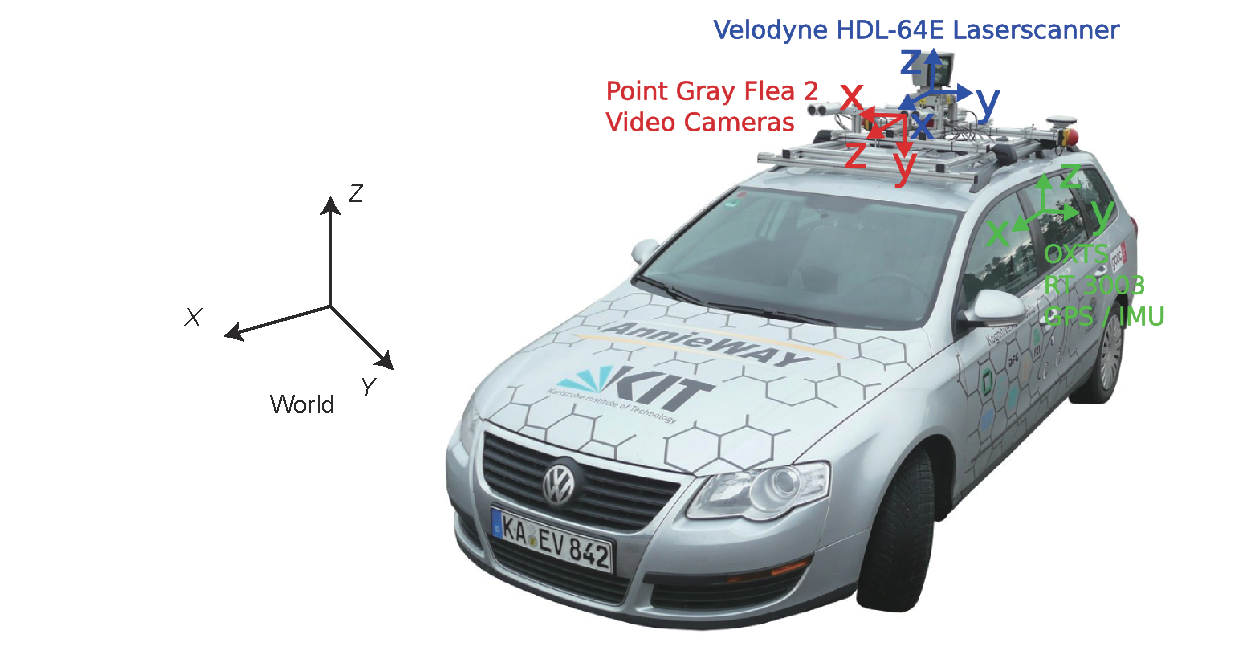
\includegraphics[width=0.7\textwidth]{math-basics/coordinate-system.pdf}
	\caption{The body and world coordinate systems of a typical autonomous vehicle sensors}
	\label{fig:corrdinate-system}
\end{figure}

An autonomous vehicle is equipped with various types of sensors. We typically assume that each sensor has its own reference frame, and their respective axis directions are defined according to the usage habits of each sensor. For example, in Figure~\ref{fig:corrdinate-system}, the IMU, 64-line lidar, and camera of the vehicle all define their own reference frames. The vehicle body generally uses the \textbf{front-left-up}\footnote{The convention "front-left-up" refers to the $X$ axis pointing forward, the $Y$ axis pointing left, and the $Z$ axis pointing up, following the right-hand rule. The convention for "right-front-up" is analogous.} or \textbf{right-front-up} order to define its coordinate system, while the camera coordinate system commonly adopts the \textbf{right-down-front} order. Consequently, there exist rotation and translation relationships between the coordinate systems of various sensors, which we characterize using rotation matrices and translation vectors.

Assuming a point $\mathbf{p}$ in the world coordinate system has coordinates $\mathbf{p}_w$, and its coordinates in the vehicle body coordinate system are $\mathbf{p}_b$, then we define the rotation matrix $\mathbf{R}_{wb}$ and the translation vector $\mathbf{t}_{wb}$, such that:

\begin{equation}
	\mathbf{p}_w = \mathbf{R}_{wb} \mathbf{p}_b + \mathbf{t}_{wb},
\end{equation}

It is crucial for readers to understand the approach here. The key points are as follows:
\begin{enumerate}
	\item Firstly, we define the transformation relationship between \textbf{coordinates}. $\mathbf{R}_{wb}$ and $\mathbf{t}_{wb}$ are used to handle coordinate transformations between vectors. Some materials deal with transformations between \textbf{coordinate axes} (or bases), interpreting rotation and translation as a transformation of a \textbf{coordinate axis} from one position to another. This definition is opposite to that of this book\footnote{One deals with transformations of coordinates, while the other deals with transformations of bases. Readers should be cautious.}, so please be careful.
	\item We can directly write $\mathbf{R}_{wb}, \mathbf{t}_{wb}$ as a \textbf{transformation matrix} $\mathbf{T}_{wb}$, expressing coordinate transformations in homogeneous form:
	\begin{equation}
		\mathbf{p}_w = \mathbf{T}_{wb} \mathbf{p}_{b}.
	\end{equation}
	This transforms the discussion into properties of the transformation matrix $\mathbf{T}$. The specific form of $\mathbf{T}$ is:
	\begin{equation}
		\mathbf{T}_{wb} = \begin{bmatrix}
			\mathbf{R}_{wb} & \mathbf{t}_{wb} \\
			\mathbf{0} & 1
		\end{bmatrix} \in \mathbb{R}^{4 \times 4}.
	\end{equation}s
	However, since the subsequent discussion will involve the IMU, which does not directly measure the differential of $\mathbf{T}$, we prefer to separate $\mathbf{R}$ and $\mathbf{t}$ rather than express them in the form of a transformation matrix.
	\item Our subscript reading order is \textbf{from right to left}, meaning the subscript $wb$ is right-multiplied with $b$ to obtain variables in the $w$ system. This makes writing and reading more fluid and intuitive. Different books handle the superscript and subscript of coordinate systems differently. Some write them on the left, some write them above, and some books even have four different markings (superscript, subscript, left, right) for one variable. This book uniformly uses the subscript $wb$ to define various variables. Since all variables have the subscript $wb$, we omit these subscripts in the vast majority of content to strive for simplicity. We also need to discuss various variables at different times or iteration numbers, which will introduce subscripts related to time or iteration numbers. If combined with coordinate system subscripts, readers would have to face a large number of formulas with various superscripts and subscripts.
\end{enumerate}

All three-dimensional rotation matrices form the \textbf{Special Orthogonal Group} ($\mathrm{SO}(3)$). It is a $3 \times 3$ real matrix that satisfies:
\begin{itemize}
	\item The rotation matrix is an orthogonal matrix: $\mathbf{R}^\top = \mathbf{R}^{-1}$.
	\item The determinant of the rotation matrix is 1: $\det(\mathbf{R}) = 1$.
\end{itemize}

Additionally, a rotation matrix can also be represented by \textbf{quaternions} or \textbf{rotation vectors}. Below, we will review their definitions and conversion relationships.

\subsection{Rotation Vectors}
Rotation vectors, also known as \textbf{angle-axis}, correspond to the Lie algebra $\mathfrak{so}(3)$ of $\mathrm{SO}(3)$. Since $\mathfrak{so}(3)$ is the tangent space of $\mathrm{SO}(3)$, as we will see later, rotation vectors can also be used to express angular velocities.

Let's denote a rotation vector as $\mathbf{w} \in \mathbb{R}^3$, and it can be decomposed into direction and magnitude: $\mathbf{w}=\theta \mathbf{n}$. The conversion relationship from rotation vector to rotation matrix can be described by \textbf{Rodrigues' formula} or the exponential map on $\mathrm{SO}(3)$:

\begin{equation}
	\label{eq:rogridues}
	\mathbf{R} = \cos \theta \mathbf{I} + \left( {1 - \cos \theta } \right) \mathbf{n}{\mathbf{n}^\top} + \sin \theta 
	{ \mathbf{n}^ \wedge } = \exp(\mathbf{w}^\wedge).
\end{equation}

Here, $\exp$ can also be expanded using Taylor series and simplified to the formula on the left. To simplify notation, we denote the uppercase $\mathrm{Exp}$ as:

\begin{equation}
	\mathrm{Exp}(\mathbf{w}) = \exp(\mathbf{w}^\wedge),
\end{equation}
which eliminates one $^\wedge$ symbol, making the formula appear more concise in complex expressions.

Conversely, the conversion relationship from rotation matrix to rotation vector can be described by the logarithmic map:

\begin{equation}
	\mathbf{w} = \log (\mathbf{R}) ^ \vee = \mathrm{Log}(\mathbf{R}).
\end{equation}

The computation method for the angle-axis is as follows. For the angle $\theta$, we have:

\begin{equation}
	\label{eq:R2theta}
	\theta = \arccos \left( \frac{\mathrm{tr}(\mathbf{R}) - 1}{2} \right).
\end{equation}

And the axis $\mathbf{n}$ is the unit eigenvector of $\mathbf{R}$ corresponding to the eigenvalue 1:

\begin{equation}
	\label{eq:R2n}
	\mathbf{R} \mathbf{n} = \mathbf{n}.	
\end{equation}

\subsection{Quaternions}
Three-dimensional rotations can also be described by unit quaternions. Quaternions, also known as expanded complex numbers, consist of a real part and three imaginary parts. This book uses Hamiltonian quaternions\footnote{According to different tastes, there are slight variations in the definition of quaternions. Hamiltonian is the most common and intuitive way of defining quaternions.}, defined as:

\begin{equation}
	\mathbf{q} = q_0 + q_1 i + q_2 j + q_3 k,
\end{equation}

where $q_0$ is the real part, and $q_1, q_2, q_3$ are the imaginary parts. The imaginary units $i, j, k$ satisfy the following multiplication rules:

\begin{equation}
	\label{eq:quaternionVirtual}
	\left\{ \begin{array}{l}
		{i^2} = {j^2} = {k^2} =  - 1\\
		ij = k,ji =  - k\\
		jk = i,kj =  - i\\
		ki = j,ik =  - j
	\end{array} \right. .
\end{equation}

To simplify notation, the three imaginary parts can be represented as a vector, and the quaternion can be expressed as a combination of scalar part $s$ and vector part $\mathbf{v}$:

\begin{equation}
	\mathbf{q} = [s, \mathbf{v}]^\top.
\end{equation}

Using the vector part, a compact form of quaternion multiplication can be written.

Following the multiplication rules of quaternions, several commonly used quaternion calculation methods can be derived. We list them below.
\begin{enumerate}
	\item \emph{Addition and Subtraction}
	
	The addition and subtraction of quaternions $\mathbf{q}_a$ and $\mathbf{q}_b$ are given by:
	\begin{equation} 	
		\mathbf{q}_a \pm \mathbf{q}_b = \left[ s_a \pm s_b, \mathbf{v}_a \pm \mathbf{v}_b \right]^\top.
	\end{equation}
	
	\item \emph{Multiplication}
	
	Multiplication involves multiplying each term of $\mathbf{q}_a$ by each term of $\mathbf{q}_b$ and then summing them up, while following the rules defined by Equation \eqref{eq:quaternionVirtual}. It can be expressed as:
	\begin{equation}
		\begin{aligned}
			\mathbf{q}_a \mathbf{q}_b &= {s_a}{s_b} - {x_a}{x_b} - {y_a}{y_b} - {z_a}{z_b}\\
			&+ \left( {{s_a}{x_b} + {x_a}{s_b} + {y_a}{z_b} - {z_a}{y_b}} \right)i\\
			&+ \left( {{s_a}{y_b} - {x_a}{z_b} + {y_a}{s_b} + {z_a}{x_b}} \right)j\\
			&+ \left( {{s_a}{z_b} + {x_a}{y_b} - {y_a}{x_b} + {z_a}{s_b}} \right)k.
		\end{aligned}
	\end{equation}
	
	Though slightly complex, this form is well-structured. Expressing it in vector form and using inner and outer product operations results in a more concise expression:
	\begin{equation}
		\mathbf{q}_a \mathbf{q}_b = \left[ s_a s_b - \mathbf{v}_a^\top \mathbf{v}_b, s_a\mathbf{v}_b + s_b\mathbf{v}_a 
		+ \mathbf{v}_a \times \mathbf{v}_b \right]^\top.
	\end{equation}
	
	Under this definition of multiplication, the product of two real quaternions is still real, which is consistent with complex numbers. However, note that quaternion multiplication is usually non-commutative due to the presence of the cross-product term, unless $\mathbf{v}_a$ and $\mathbf{v}_b$ are collinear in $\mathbb{R}^3$, in which case the cross-product term becomes zero.
	
	This book does not deliberately distinguish between standard multiplication and quaternion multiplication. Some materials may use symbols such as $\otimes$ to differentiate quaternion multiplication, but this book consistently uses standard multiplication. Quaternions are not multiplied with ordinary vectors or matrices, so **the meaning of multiplication should be clear**.
	
	\item \emph{Norm}
	
	The norm of a quaternion is defined as:
	\begin{equation}
		\| \mathbf{q}_a \| = \sqrt{ s_a^2 + x_a^2 + y_a^2 + z_a^2 }.
	\end{equation}
	It can be verified that the norm of the product of two quaternions equals the product of their norms, which ensures that the product of unit quaternions remains a unit quaternion:
	\begin{equation}
		\| \mathbf{q}_a \mathbf{q}_b \| = \|\mathbf{q}_a \| \| \mathbf{q}_b \|.
	\end{equation}
	
	\item \emph{Conjugate}
	
	The conjugate of a quaternion is obtained by negating the imaginary parts:
	\begin{equation}
		\mathbf{q}_a^* = s_a - x_ai - y_aj - z_ak = [s_a, -\mathbf{v}_a]^\top.
	\end{equation}
	Multiplying a quaternion by its conjugate yields a real quaternion with a real part equal to the square of its norm:
	\begin{equation}
		\mathbf{q}^* \mathbf{q} = \mathbf{q} \mathbf{q}^* = [s^2+\mathbf{v}^\top \mathbf{v}, \mathbf{0} ]^\top.
	\end{equation}
	
	\item \emph{Inverse}
	
	The inverse of a quaternion is given by:
	\begin{equation}
		\label{eq:quaternionInverse}
		\mathbf{q}^{-1} = \mathbf{q}^* / \| \mathbf{q} \| ^2.
	\end{equation}
	According to this definition, the product of a quaternion and its inverse yields a real quaternion $\mathbf{1}$:
	\begin{equation}
		\mathbf{q} \mathbf{q}^{-1} = \mathbf{q}^{-1} \mathbf{q} = \mathbf{1}.
	\end{equation}
	
	If $\mathbf{q}$ is a unit quaternion, its inverse and conjugate are the same. Moreover, the inverse of a product obeys a property similar to matrices:
	\begin{equation}
		\left( \mathbf{q}_a \mathbf{q}_b \right)^{-1} = \mathbf{q}_b^{-1} \mathbf{q}_a^{-1}.
	\end{equation}
	
	\item \emph{Scalar Multiplication}
	
	Similar to vectors, quaternions can be multiplied by scalars:
	\begin{equation}
		k \mathbf{q} = \left[ ks, k\mathbf{v} \right]^\top.
	\end{equation}
\end{enumerate}


\subsubsection{Representing Rotation with Quaternions}
Rotation of a point can be expressed using quaternions. Let's assume a three-dimensional point in space $\mathbf{p} = [x,y,z]\in \mathbb{R}^3$, and a rotation specified by a unit quaternion $\mathbf{q}$. The point $\mathbf{p}$ undergoes a rotation to become $\mathbf{p}'$. If described using matrices, then $\mathbf{p}'=\mathbf{R} \mathbf{p}$. But how can we express this relationship using quaternions?

Firstly, represent the three-dimensional space point using a quaternion:
\begin{equation}
\mathbf{p} = [0, x, y, z]^\top = [0, \mathbf{v}]^\top.
\end{equation}
This is equivalent to associating the three imaginary parts of the quaternion with the three axes in space. Then, the rotated point $\mathbf{p}'$ can be expressed as the following product:
\begin{equation}\label{eq:rotate-with-quaternion}
	\mathbf{p}' = \mathbf{q} \mathbf{p} \mathbf{q}^{-1}.
\end{equation}
Here, the multiplication is quaternion multiplication, resulting in another quaternion. Finally, extract the imaginary part of $\mathbf{p}'$ to obtain the coordinates of the point after rotation. It can be verified that the real part of the computed result is 0, hence it is a pure imaginary quaternion.

\subsubsection{Conversion from Quaternion to Rotation Matrix and Rotation Vector}
Any unit quaternion describes a rotation, which can also be described using a rotation matrix or rotation vector. Now, let's examine the relationship between quaternions and rotation vectors, rotation matrices.

Before diving into that, it's worth mentioning that quaternion multiplication can also be expressed as a form of matrix multiplication. Let $\mathbf{q}=[s,\mathbf{v}]^\top$ be a quaternion. Define the following symbols $^{+}$ and $^{\oplus}$ as follows\cite{Barfoot2011}:
\begin{equation}
	\mathbf{q}^{+}=\left[\begin{array}{cc}
		s&-\mathbf{v}^\top \\
		\mathbf{v}&s\mathbf{I}+\mathbf{v}^{\wedge}
	\end{array}\right],\quad 
	\mathbf{q}^{\oplus}=
	\left[\begin{array}{cc}
		s & -\mathbf{v}^\top \\
		\mathbf{v} & s\mathbf{I}-\mathbf{v}^{\wedge}
	\end{array}\right],
\end{equation}
where these symbols map quaternions into a $4\times 4$ matrix. Thus, quaternion multiplication can be written in matrix form as follows:
\begin{equation}
	\mathbf{q}_1^ + {\mathbf{q}_2} = \left[ {\begin{array}{*{20}{c}}
			s_1&-\mathbf{v}_1^\top\\
			\mathbf{v}_1 & s_1 \mathbf{I} + \mathbf{v}_1^\wedge
	\end{array}} \right]\left[ {\begin{array}{*{20}{c}}
			{{s _2}} \\
			{{\mathbf{v} _2}}
	\end{array}} \right] = \left[ {\begin{array}{*{20}{c}}
			{ - \mathbf{v} _1^\top{\mathbf{v} _2} + {s _1}{s _2}} \\ 
			{{s _1}{\mathbf{v} _2} + {s _2}{\mathbf{v} _1} + \mathbf{v} _1^ \wedge {\mathbf{v} _2}}
	\end{array}} \right] = \mathbf{q}_1 \mathbf{q}_2.
\end{equation}
Similarly, it can be proven that:
\begin{equation}
	\mathbf{q}_1 \mathbf{q}_2 = \mathbf{q}_1^{+} \mathbf{q}_2 = \mathbf{q}_2^{\oplus} \mathbf{q}_1.
\end{equation}

Then, let's consider the problem of rotating a point in space using quaternions. According to the previous discussion, we have:
\begin{equation}\label{eq:quaternion-to-rotation-matrix-derive}
	\begin{split}
		\mathbf{p}' &= \mathbf{q} \mathbf{p} \mathbf{q}^{-1} = \mathbf{q}^+ \mathbf{p}^+ \mathbf{q}^{-1} \\
		&= \mathbf{q}^+ \mathbf{q}^{{-1}^{\oplus}} \mathbf{p}.
	\end{split}
\end{equation}
Substituting the matrices corresponding to the two symbols, we obtain:
\begin{equation}
	{\mathbf{q}^ + }{\left( {{\mathbf{q}^{ - 1}}} \right)^ \oplus } = \left[ \begin{array}{*{20}{c}}
		s&-\mathbf{v}^\top\\
		\mathbf{v}&s\mathbf{I}+\mathbf{v}^\wedge 
	\end{array} \right]\left[\begin{array}{*{20}{c}}
		s&{\mathbf{v} ^\top}\\
		{ - \mathbf{v} }&{s\mathbf{I} + \mathbf{v} ^ \wedge }
	\end{array} \right] = \left[ \begin{array}{*{20}{c}}
		1&\mathbf{0} \\
		\mathbf{0}^\top&\mathbf{v}\mathbf{v}^\top + {s^2} \mathbf{I} + 2s\mathbf{v} ^ \wedge + {(\mathbf{v} ^ 
			\wedge)}^2 
	\end{array} \right].
\end{equation}
Since both $\mathbf{p}'$ and $\mathbf{p}$ are purely imaginary quaternions, the lower right corner of this matrix actually gives the transformation from quaternion to rotation matrix:
\begin{equation}
	\mathbf{R} = \mathbf{v} \mathbf{v}^\top + {s^2} \mathbf{I} + 2s\mathbf{v} ^ \wedge + {(\mathbf{v} ^ \wedge)}^2.
\end{equation}
To obtain the conversion formula from quaternion to rotation vector, take the trace of both sides of the above equation:
\begin{equation}
	\begin{aligned}
		\mathrm{tr}(\mathbf{R}) &= \mathrm{tr}(\mathbf{v}\mathbf{v}^\top) + 3s^2 + 2s \cdot 0 + 
		\mathrm{tr}((\mathbf{v}^\wedge)^2) \\
		&= v_1^2+v_2^2+v_3^2 + 3s^2 - 2(v_1^2+v_2^2+v_3^2) \\
		&= (1-s^2) + 3s^2 -2(1-s^2)\\
		&= 4s^2 -1.
	\end{aligned}
\end{equation}
Also, from Eq.\eqref{eq:R2theta}, we have:
\begin{equation}
	\begin{aligned}
		\theta &= \arccos(\frac{\mathrm{tr}(\mathbf{R})-1}{2}) \\
		&=\arccos(2s^2-1).
	\end{aligned}
\end{equation}
Thus,
\begin{equation}
	\cos \theta =2s^2-1=2 \cos^2 \frac{\theta}{2} -1,
\end{equation}
so:
\begin{equation}
	\theta = 2 \arccos s.
\end{equation}
Regarding the rotation axis, if we substitute $\mathbf{q}$'s imaginary part for $\mathbf{p}$ in Eq.\eqref{eq:quaternion-to-rotation-matrix-derive}, it's easy to see that the vector formed by the imaginary part of $\mathbf{q}$ remains fixed during rotation, constituting the rotation axis. Thus, by normalizing it by its magnitude, we obtain the rotation axis. In summary, the conversion formula from quaternion to rotation vector can be expressed as follows:
\begin{equation}
	\label{eq:rotationVector2Quaternion}
	\begin{cases}
		\theta  = 2\arccos s\\
		{\left[ {{n_x},{n_y},{n_z}} \right]^\top} = \mathbf{v}^\top /{\sin 
			\frac{\theta }{2}}
	\end{cases} .
\end{equation}

Since quaternions require only four values to represent rotation, most programs choose quaternions as the underlying representation for rotations. They may provide interfaces for matrix operations, such as the previously mentioned $\vee$ or $\log$ operations, or interfaces for quaternions, such as retrieving the four components of a quaternion, and so on. When using these programs, we can simply use these matrix interfaces without concerning ourselves with their underlying storage format.

\subsection{Lie Group and Lie Algebra}
Three-dimensional rotations form the three-dimensional rotation group $\mathrm{SO}(3)$, with its corresponding Lie algebra denoted as $\mathfrak{so}(3)$; three-dimensional transformations form the three-dimensional transformation group $\mathrm{SE}(3)$, with its corresponding Lie algebra denoted as $\mathfrak{se}(3)$.

The mapping from Lie algebra elements to Lie group elements is known as the exponential mapping. For $\mathfrak{so}(3)$ to $\mathrm{SO}(3)$, the exponential mapping is given by:
\begin{equation}\label{key}
	\exp(\boldsymbol{\phi}^\wedge) = \mathbf{R},
\end{equation}
where the specific computation is provided by the Rodrigues' formula \eqref{eq:rogridues}. The inverse mapping, known as the logarithm mapping, is denoted as:
\begin{equation}\label{key}
	\boldsymbol{\phi} = \log(\mathbf{R})^\vee,
\end{equation}
with specific computation provided by equations \eqref{eq:R2theta} and \eqref{eq:R2n}.

We mainly utilize the combination of $\mathrm{SO}(3)$ with translation vectors to derive subsequent motion equations, filtering relationships, etc. We omit the introduction of $\mathrm{SE}(3)$ and $\mathfrak{se}(3)$.

\subsection{BCH Linear Approximation on $\mathrm{SO}(3)$}
The Baker-Campbell-Hausdorff (BCH) formula \cite{gilmore1974baker} provides a relationship between the addition of small quantities in the Lie algebra and the multiplication of small quantities in the Lie group, which is widely used for linearization of various functions. Here, we only present the conclusions.

In $\mathrm{SO}(3)$, for a rotation $\mathbf{R}$ (corresponding to the Lie algebra $\boldsymbol{\phi}$), left-multiplying it by a small rotation, denoted as $\Delta \mathbf{R}$, with the corresponding Lie algebra $\Delta \boldsymbol{\phi}$, results in $ \Delta \mathbf{R} \cdot \mathbf{R}$ on the Lie group. According to the BCH approximation, in the Lie algebra, it is $\mathbf{J}_l^{-1} (\boldsymbol{\phi}) \Delta \boldsymbol{\phi} + \boldsymbol{\phi}$. Thus, we can simply write:
\begin{equation}
	\exp \left( {\Delta { \boldsymbol{\phi} ^ \wedge }} \right)\exp \left( {{ \boldsymbol{\phi} ^ \wedge }} 
	\right) = \exp \left( {{{\left( { \boldsymbol{\phi}  + \mathbf{J}_l^{ - 1}\left( \boldsymbol{\phi}  \right)\Delta 
					\boldsymbol{\phi} } \right)}^ \wedge }} \right).
\end{equation}

Conversely, if we perform addition in the Lie algebra, adding $\Delta \boldsymbol{\phi}$ to $\boldsymbol{\phi}$, it can be approximated as multiplication with left and right Jacobians on the Lie group:
\begin{equation}
	\exp \left( {{{\left( { \boldsymbol{\phi}  + \Delta \boldsymbol{\phi} } \right)}^ \wedge }} \right) = \exp 
	\left( {{{\left( {{ \mathbf{J}_l} (\boldsymbol{\phi})\Delta \boldsymbol{\phi} } \right)}^ \wedge }} \right)\exp \left( {{ 
			\boldsymbol{\phi} ^ \wedge }} \right) = \exp \left( {{\boldsymbol{\phi} ^ \wedge }} \right)\exp \left( 
	{{{\left( {{\mathbf{J}_r}(\boldsymbol{\phi}) \Delta \boldsymbol{\phi} } \right)}^ \wedge }} \right).
\end{equation}

Where the left Jacobian for $\mathrm{SO}(3)$ is given by:
\begin{align}
	\mathbf{J}_l (\theta \mathbf{a}) &= \frac{\sin \theta}{\theta} \mathbf{I} + (1-\frac{\sin \theta }{\theta}) \mathbf{a} \mathbf{a}^\top + \frac{1-\cos \theta}{\theta} \mathbf{a}^\wedge \\
	\mathbf{J}_l^{ - 1}(\theta \mathbf{a}) &= \frac{\theta }{2}\cot \frac{\theta }{2} \mathbf{I} + \left( {1 - \frac{\theta 
		}{2}\cot \frac{\theta }{2}} \right) \mathbf{a} {\mathbf{a}^\top} - \frac{\theta }{2}{ \mathbf{a}^ \wedge }. 
\end{align}
And the right Jacobian for $\mathrm{SO}(3)$ is:
\begin{equation}
	\mathbf{J}_r(\boldsymbol{\phi}) =\mathbf{J}_l(-\boldsymbol{\phi}) .
\end{equation}

Since the Lie algebra $\boldsymbol{\phi}$ and $\mathbf{R}$ can be easily associated, sometimes we also simply denote $\mathbf{J}_r(\boldsymbol{\phi})$ as $\mathbf{J}_r(\mathbf{R})$ instead of $\mathbf{J}_r(\mathrm{Log}(\mathbf{R}))$. This can make the formulas look more concise. In many cases, we also omit the part inside the parentheses of $\mathbf{J}_r(\boldsymbol{\phi})$ and directly write $\mathbf{J}_r$ and $\mathbf{J}_l$.

All of the above content has been introduced in \cite{Gao2017} already. If readers are interested in their detailed derivation process, please check \cite{Gao2017}, \cite{Barfoot2016} or \cite{Sola2017}. This book will directly use the conclusions introduced above.

\section{Kinematics}
Now let's consider a three-dimensional object in motion over time. In this section, we will explore various perspectives on expressing three-dimensional kinematics, which will be correlated with subsequent chapters. Examining three-dimensional kinematics will lead to a series of interesting discussions. Join us as we delve into it.

\subsection{Kinematics from the Perspective of Lie Groups}
\label{sec:so3-kinematics}
Earlier, we discussed how the rotation and translation of an object can be described by $\mathbf{R}$ and $\mathbf{t}$, respectively (here, we omit the subscript $wb$ denoting the coordinate frame). When they vary continuously with time, they become functions of time, $\mathbf{R}(t)$ and $\mathbf{t}(t)$. Obviously, the translational part is trivial, just a function with the codomain $\mathbb{R}^3$. Therefore, we focus on the rotational part.

Let's assume that $\mathbf{R}$ varies with time, i.e., $\mathbf{R}(t)$. According to the property of $\mathbf{R}$ being an orthogonal matrix:
\begin{equation}\label{key}
	\mathbf{R}^\top \mathbf{R} = \mathbf{I},
\end{equation}
it is not difficult to observe:
\begin{equation}
	\frac{\mathrm{d}}{{\mathrm{d}t}}\left( {{\mathbf{R}^\top} \mathbf{R}} \right) = {\dot{\mathbf{R}}^\top} \mathbf{R} 
	+ {\mathbf{R}^\top}\dot{\mathbf{R}} = \mathbf{0},
\end{equation}
which implies:
\begin{equation}
	{\mathbf{R}^\top}\dot{\mathbf{R}} = -({\mathbf{R}^\top}\dot{\mathbf{R}})^\top.
\end{equation}
It can be seen that ${\mathbf{R}^\top}\dot{\mathbf{R}}$ is a skew-symmetric matrix, and a skew-symmetric matrix can be expressed in vector form using the skew-symmetric symbol $^\wedge$. Let's take $\boldsymbol{\omega}^\wedge \in \mathbb{R}^{3 \times 3} = 
{\mathbf{R}^\top}\dot{\mathbf{R}}$, then we can write $\mathbf{R}$ in the form of a differential equation:

\begin{equation}\label{eq:2.51}
	\dot{\mathbf{R}} = \mathbf{R} \boldsymbol{\omega}^\wedge.
\end{equation}

This equation is also known as the \textbf{Poisson equation}\cite{Rauch1965}. It's worth noting that we could also start from $\mathbf{R} \mathbf{R}^\top = \mathbf{I}$, define $\boldsymbol{\omega}^\wedge = \dot{\mathbf{R}} \mathbf{R}^\top$, and obtain the result $\dot{\mathbf{R}} = \boldsymbol{\omega}^\wedge\mathbf{R}$. These two forms are essentially equivalent, just different in appearance.

If we only consider instantaneous changes, then at a fixed time $t$, $\boldsymbol{\omega}$ can be considered constant. In physical terms, we call $\boldsymbol{\omega}$ the \textbf{instantaneous angular velocity}. Given an initial rotation matrix $\mathbf{R}(t_0)$ at time $t_0$, the solution to the above differential equation is:
\begin{equation}\label{eq:2.52}
	\mathbf{R}(t) = \mathbf{R}(t_0) \exp(\boldsymbol{\omega}^\wedge (t-t_0)).
\end{equation}

If readers are familiar with the knowledge of Lie groups and Lie algebras, it's easy to recognize that Equation \eqref{eq:2.52} represents the exponential mapping on $\mathrm{SO}(3)$. Let $\Delta t = t - t_0$, then this equation can also be written as:
\begin{equation}\label{eq:2.53}
	\mathbf{R}(t) = \mathbf{R}(t_0) \mathrm{Exp}(\boldsymbol{\omega} \Delta t).
\end{equation}

From another perspective, we can also expand $\mathbf{R}(t)$ around time $t_0$ using Taylor series, and the first-order approximation is:
\begin{equation}\label{eq:2.54}
	\begin{array}{ll}
		\mathbf{R}(t_0 + \Delta t) &\approx \mathbf{R}(t_0) + \dot{\mathbf{R}}(t_0) \Delta t  \\
		& = \mathbf{R}(t_0) + \mathbf{R}(t_0) \boldsymbol{\omega}^\wedge \Delta t \\ 
		& = \mathbf{R}(t_0)(\mathbf{I} + \boldsymbol{\omega}^\wedge \Delta t).
	\end{array}
\end{equation}

This reveals the approximate form of the exponential mapping:
\begin{equation}
	\mathrm{Exp}( \boldsymbol{\omega} \Delta t) = \mathbf{I} + \boldsymbol{\omega}^\wedge \Delta t+ 
	\frac{1}{2}(\boldsymbol{\omega} ^\wedge \Delta t)^2 + \ldots
\end{equation}

By comparing the above equations, we can see that:
\begin{enumerate}
	\item Equation \eqref{eq:2.53} is the discrete-time form of Equation \eqref{eq:2.52}.
	\item Equation \eqref{eq:2.54} is the linear approximation of Equation \eqref{eq:2.53}.
\end{enumerate}

These two sets of equations are very useful in dealing with angular velocities, and we will continue to use them in the subsequent discussion.

\subsection{Kinematics from the Perspective of Quaternions}

Now let's examine how the kinematic equations change if we use quaternions to represent rotations. This is an alternative description of the same problem from a different perspective. Investigating this issue can help us establish connections between different mathematical representations. We know that the rotation of a vector by quaternions should take the form given by Equation \eqref{eq:quaternion-to-rotation-matrix-derive}, and quaternions themselves carry the unit constraint $\mathbf{q}\mathbf{q}^*=\mathbf{q}^*\mathbf{q} = \mathbf{1}$. Similar to the case of $\mathrm{SO}(3)$, starting from $\mathbf{q}^* 
\mathbf{q} = \mathbf{1}$, if we differentiate both sides with respect to time, we get:
\begin{equation}\label{key}
	\dot{\mathbf{q}^*} \mathbf{q} +\mathbf{q}^* \dot{\mathbf{q}} = \mathbf{0},
\end{equation}
which leads to:
\begin{equation}\label{key}
	\mathbf{q}^* \dot{\mathbf{q}} = - \dot{\mathbf{q}^*} \mathbf{q} = -(\mathbf{q}^* \dot{\mathbf{q}})^*.
\end{equation}
Thus, $\mathbf{q}^* 
\dot{\mathbf{q}}$ is a pure quaternion (with zero real part). We can denote a pure quaternion as $\boldsymbol{\varpi } = 
[0, \underbrace{\boldsymbol{\omega}_1, \boldsymbol{\omega}_2, 
	\boldsymbol{\omega}_3}_{\boldsymbol{\omega}}]^\top \in \mathcal{Q}$, so we have:
\begin{equation}
	\mathbf{q}^* \dot{\mathbf{q}} = \boldsymbol{\varpi}.
\end{equation}
Multiplying both sides by $\mathbf{q}$, we get:
\begin{equation}\label{eq:2.59}
	\dot{\mathbf{q}} = \mathbf{q} \boldsymbol{\varpi}.
\end{equation}

This equation is very similar to Equation \eqref{eq:2.51}. Analogous to the case of $\mathrm{SO}(3)$, we can also discuss the instantaneous angular velocity, Lie algebra, exponential mapping, and logarithmic mapping near time $t$. When considering instantaneous changes, we can treat $\boldsymbol{\varpi}$ as a constant value, so the solution to the above differential equation is:
\begin{equation}\label{key}
	\mathbf{q}(t) = \mathbf{q}(t_0) \exp(\boldsymbol{\varpi} \Delta t),
\end{equation}
where we used the quaternion exponential mapping. Let's take a brief pause in the derivation and introduce the quaternion exponential mapping in the usual sense.

For any pure quaternion $\boldsymbol{\varpi} = [0, \boldsymbol{\omega}]^\top \in 
\mathcal{Q}$, its exponential mapping is defined as:
\begin{equation}\label{key}
	\exp \left( \boldsymbol{\varpi}  \right) = \sum\limits_{k = 0}^\infty  {\frac{1}{{k!}}{\boldsymbol{\varpi}^k}} .
\end{equation}

Separating its direction and magnitude, let $\boldsymbol{\varpi} =  \mathbf{u} \theta$, where $\theta$ is the magnitude of $\boldsymbol{\varpi}$ and $\mathbf{u}$ is the unit imaginary quaternion. Since $\mathbf{u}$ is an unit imaginary quaternion, we have:
\begin{equation}\label{key}
	\mathbf{u}^2 = -\mathbf{1}, \quad \mathbf{u}^3 = -\mathbf{u},
\end{equation}
which is similar to the self-multiplication property of unit imaginary numbers and can be used to simplify higher-order terms. Using this property, we can derive:
\begin{equation}\label{key}
	\begin{aligned}
		\exp \left( {\mathbf{u}\theta } \right) &= 1 + \mathbf{u}\theta  - \frac{1}{{2!}}{\theta ^2} - \frac{1}{{3!}}{\theta 
			^3}\mathbf{u} + \frac{1}{{4!}}{\theta ^4} +  \ldots \\
		&= \underbrace{\left( {1 - \frac{1}{{2!}}{\theta ^2} + \frac{1}{{4!}}{\theta ^4} -  \ldots } \right)}_{\cos 
			\theta} + \underbrace{\left( {\theta  - \frac{1}{{3!}}{\theta ^3} + \frac{1}{{5!}}{\theta ^5} -  \ldots } 
			\right)}_{\sin \theta}\mathbf{u} \\
		&= \cos \theta  + \mathbf{u}\sin \theta .
	\end{aligned}
\end{equation}

This formula is very similar to Euler's formula for complex numbers:
\begin{equation}\label{key}
	\exp(i \theta) = \cos \theta + i \sin \theta,
\end{equation}
and it's indeed its extension to quaternions.

Substituting the pure imaginary $\boldsymbol{\varpi}$, we obtain:
\begin{equation}\label{eq:2.66}
	\exp(\boldsymbol{\varpi}) = [\cos\theta, \mathbf{u} \sin \theta] ^\top.
\end{equation}
Also, because $\boldsymbol{\varpi}$ is an imaginary quaternion, we have:
\begin{equation}\label{key}
	\| \exp(\boldsymbol{\varpi}) \| = \cos^2 \theta + \sin^2 \theta \| \mathbf{u} \|^2 = 1.
\end{equation}
So, the result of the exponential mapping of an imaginary quaternion is a unit quaternion, which is also a mapping relationship between unit quaternions and pure quaternions. We can also think of the imaginary quaternion $\boldsymbol{\varpi}$ as a quaternion form of the Lie algebra. Therefore, an obvious question arises: what is the relationship between the quaternion form of the Lie algebra and the rotation vector form of the Lie algebra?

\subsection{Conversion between Lie Algebra of Quaternions and Rotation Vectors}
Consider a rotation matrix $\mathbf{R}$ and its rotation vector $\boldsymbol{\phi}$. Obviously, their relationship is described by the exponential mapping:
\begin{equation}
	\mathbf{R} = \mathrm{Exp} (\boldsymbol{\phi}) = \mathrm{Exp}(\theta \mathbf{n}),
\end{equation}
where $\mathbf{n}$ is the direction of the rotation vector and $\theta$ is its magnitude. We also assume that this rotation can be expressed by $\mathbf{q} = 
\mathrm{Exp} (\boldsymbol{\varpi})$, where $\boldsymbol{\varpi}$ is a pure imaginary quaternion $[0, 
\boldsymbol{\omega}]^\top$. Now let's examine the transformation relationship between these two representations.

From Equation \eqref{eq:rotationVector2Quaternion}, we know that the quaternion corresponding to $\mathbf{R}$ is:
\begin{equation}\label{key}
	\mathbf{q} = [\cos \frac{\theta}{2}, \mathbf{n} \sin \frac{\theta}{2}],
\end{equation}
By comparing with Equation \eqref{eq:2.66}, it's easy to see the relationship between $\boldsymbol{\varpi}$ and $\boldsymbol{\phi}$:
\begin{equation}\label{key}
	\boldsymbol{\varpi} = [0, \frac{1}{2} \boldsymbol{\phi}]^\top, \quad \text{or} \  
	\boldsymbol{\omega} = \frac{1}{2} \boldsymbol{\phi}.
\end{equation}

We miraculously discover that the angular velocity expressed by quaternions is exactly half of the $\mathrm{SO}(3)$ Lie algebra! This is because when using quaternions to rotate a vector, we need to multiply corresponding parts twice. Due to this ``half'' relationship, the Lie algebra corresponding to quaternions is slightly different from $\mathfrak{so}(3)$. To maintain the continuity of derivation and writing, we use a unified $\mathrm{Exp}$ relationship to combine the two definitions. In summary, for a three-dimensional instantaneous angular velocity (or the update quantity of an optimization function) $\boldsymbol{\omega} \in \mathbb{R}^3$, we define its kinematic form on $\mathrm{SO}(3)$ as:
\begin{equation}\label{eq:rotation-matrix-kinematics}
	\dot{\mathbf{R}} = \mathbf{R} \boldsymbol{\omega}^\wedge
\end{equation}
Its corresponding exponential mapping is:
\begin{equation}\label{key}
	\mathbf{R} = \mathrm{Exp} (\boldsymbol{\omega}) = \exp(\boldsymbol{\omega}^\wedge),
\end{equation}
or, if this quantity is the update amount of a pure imaginary quaternion (typically obtained from solving an optimization function), then the corresponding quaternion should only update half of it. According to the definition in Equation \eqref{eq:2.59}, the quaternion kinematic equation and exponential mapping can be written as:
\begin{equation}\label{eq:quaternion-kinematics}
	\dot{\mathbf{q}} = \frac{1}{2} \mathbf{q} [0, \boldsymbol{\omega}]^\top,
\end{equation}
which can usually be simplified as\footnote{Note that the meaning of $\boldsymbol{\omega}$ has changed here. In the previous equation, it was a three-dimensional vector, while in the next equation, it is a quaternion.}:
\begin{equation}
	\dot{\mathbf{q}} = \frac{1}{2} \mathbf{q} \boldsymbol{\omega},
\end{equation}
Here, the coefficient $1/2$ is used to unify the definition of angular velocity on $\mathrm{SO}(3)$ with quaternion angular velocity, so this equation differs from Equation \eqref{eq:2.59}. Readers should also note that this equation implies that the three-dimensional vector $\boldsymbol{\omega}$ is first converted to a quaternion before multiplying with $\mathbf{q}$, rather than directly multiplying $\mathbf{q}$ by $\boldsymbol{\omega}$.

The quaternion exponential mapping can also be written similarly as:
\begin{equation}\label{key}
	\mathbf{q} = \exp(\frac{1}{2} [0, \boldsymbol{\omega}]^\top) \buildrel \Delta \over = 
	\mathrm{Exp}(\boldsymbol{\omega}).
\end{equation}

If $\boldsymbol{\omega}$ is small, then $\cos(\frac{\theta}{2}) \approx 1, \mathbf{n} \sin \frac{\theta}{2} \approx \mathbf{n} \frac{\theta}{2}$, and the exponential mapping has a simplified form:
\begin{equation}\label{key}
	\mathrm{Exp}(\boldsymbol{\omega}) \approx [1, \frac{1}{2} \boldsymbol{\omega}],
\end{equation}

So the quaternion update formula can be simplified as\footnote{In this equation, there is no need to change the definition of $\boldsymbol{\omega}$, it is still a three-dimensional vector.}:
\begin{equation}\label{eq:2.76}
\mathbf{q} \mathrm{Exp}(\boldsymbol{\omega}) \approx \mathbf{q} [1, \frac{1}{2} \boldsymbol{\omega}],
\end{equation}

However, a significant disadvantage of this equation compared to the update equation on $\mathrm{SO}(3)$ is that the quaternion on the right-hand side is not a unit quaternion, so after long-term updates, it needs to be re-normalized \cite{Sola2017}. This problem does not exist for rotation matrices, as $\mathrm{Exp}(\boldsymbol{\omega})$ is always a rotation matrix.

Thus far, we have introduced the kinematics from the perspectives of $\mathrm{SO}(3)$ and quaternions, as well as their conversion relationship. With this relationship, we can use either rotation matrices or quaternions when writing the motion equations of a vehicle or when calculating the Jacobian matrices of optimization problems, just remember the coefficient of $1/2$. We can also mix quaternions and rotation matrices, just remember that when updating variables, quaternions only need to be updated by half.

In addition, we can also consider kinematics at the level of the Lie algebra $\mathfrak{so}(3)$. For the translation part, it can be viewed as independent three-dimensional variables or collectively considered in $\mathrm{SE}(3)$. In practice, these expressions are interchangeable without essential differences, but there may be differences in the ease of operation. We introduce several other expressions in this section, but only one of them will be detailed in subsequent chapters.

\subsection{Other Kinematic Representations}

\subsubsection{Kinematics on $\mathfrak{so}(3)$}
To give some physical meaning to mathematical symbols, we will use $\boldsymbol{\omega}$ to express angular velocity and $\boldsymbol{\phi}$ to express rotation vectors in the future. The Rodrigues formula tells us that $\mathbf{R} = \mathrm{Exp}(\boldsymbol{\phi})$. Now we want to examine the derivative of $\boldsymbol{\phi}$ with respect to time and its relationship with the instantaneous angular velocity $\boldsymbol{\omega}$.

The BCH formula gives the relationship between increments on the Lie group and the Lie algebra. Assuming that at time $t$ to $t+\Delta 
t$, $\boldsymbol{\phi}(t)$ changes to $\boldsymbol{\phi}(t) + \Delta 
\boldsymbol{\phi}$ on $\mathfrak{so}(3)$, and at the same time $\mathrm{SO}(3)$ changes from $\mathbf{R}$ to $\mathbf{R} \cdot \Delta 
\mathbf{R}$, then according to the BCH approximation, we have:
\begin{equation}\label{key}
	\Delta \mathbf{R} = \mathrm{Exp}( \mathbf{J}_r \Delta \boldsymbol{\phi}),
\end{equation}
On the $\mathrm{SO}(3)$ level, according to the definition of angular velocity, we have $\dot{\mathbf{R}} = \mathbf{R} 
\boldsymbol{\omega}^\wedge$, so:
\begin{equation}\label{key}
	\begin{array}{ll}
		\mathbf{R}\boldsymbol{\omega}^\wedge &= \dot{\mathbf{R}} = \mathop {\lim }\limits_{\Delta t \to 0} 
		\frac{{\mathbf{R}\left( {t + \Delta t} \right) - \mathbf{R}\left( t \right)}}{{\Delta t}}\\
		&\approx \mathop {\lim }\limits_{\Delta t \to 0} \frac{{\mathbf{R}\left( t \right)\mathrm{Exp}\left( 
				{{\mathbf{J}_r}\Delta \boldsymbol{\phi} } \right) - \mathbf{R}\left( t \right)}}{{\Delta t}}\\
		&\approx \mathop {\lim }\limits_{\Delta t \to 0} \frac{{\mathbf{R}\left( t \right)\left( {\mathrm{Exp}\left( 
					{{\mathbf{J}_r}\Delta \boldsymbol{\phi} } \right) - \mathbf{I}} \right)}}{{\Delta t}} = \mathbf{R} (\mathbf{J}_r \dot{\boldsymbol{\phi}})^\wedge,
	\end{array}
\end{equation}
where the last equality requires a Taylor expansion of the $\mathrm{Exp}$ function. By comparing the left and right sides, we easily obtain:
\begin{equation}
	\boldsymbol{\omega} = \mathbf{J}_r \dot{\boldsymbol{\phi}},
\end{equation}
or:
\begin{equation}\label{key}
	\dot{\boldsymbol{\phi}} = \mathbf{J}_r^{-1} \boldsymbol{\omega}.
\end{equation}
This shows the relationship between the time derivative on $\mathfrak{so}(3)$ and the instantaneous angular velocity on $\mathrm{SO}(3)$. In principle, we can also use this quantity to derive subsequent filters or optimizers. However, its physical meaning is not as intuitive as $\boldsymbol{\omega}$, so very few people actually choose this method.

\subsubsection{Kinematics on $\mathrm{SO}(3) + \mathbf{t}$}

We can incorporate linear velocity into consideration. For example, let $\mathbf{v} = \dot{\mathbf{t}}$, then the system kinematic equations can be written as:
\begin{equation}\label{key}
	\dot{\mathbf{R}} = \mathbf{R} \boldsymbol{\omega}^\wedge, \quad \dot{\mathbf{t}} = \mathbf{v}.
\end{equation}

This approach is the simplest and most intuitive, and is widely adopted.

\subsubsection{Kinematics on $\mathrm{SE}(3)$}

We can also derive kinematics on $\mathrm{SE}(3)$ and make it consistent with the exponential mapping on $\mathrm{SO}(3)$. This requires some modifications to the linear velocity part. Let the transformation matrix be:
\begin{equation}\label{key}
	\mathbf{T} = \begin{bmatrix}
		\mathbf{R} & \mathbf{t} \\
		\mathbf{0}^\top & 1
	\end{bmatrix} \in \mathrm{SE}(3),
\end{equation}
then its time derivative is:
\begin{equation}\label{key}
	\dot{\mathbf{T}} = \begin{bmatrix}
		\dot{\mathbf{R}} & \dot{\mathbf{t}} \\
		\mathbf{0}^\top & 0
	\end{bmatrix}
	= \begin{bmatrix}
		\mathbf{R} \boldsymbol{\omega}^\wedge & \mathbf{v} \\
		\mathbf{0} ^\top & 0
	\end{bmatrix}.
\end{equation}

For instance, to achieve the kinematics on $\mathrm{SE}(3)$ in the right-multiplication model, we want to obtain the form $\dot{\mathbf{T}} = \mathbf{T} \boldsymbol{\xi}^\wedge$\footnote{The $\wedge$ symbol on $\mathrm{SE}(3)$ is defined as: $\boldsymbol{\xi}^\wedge = \begin{bmatrix}
		\boldsymbol{\phi}^\wedge & \boldsymbol{\rho}^\wedge \\ \mathbf{0}^\top & 0
	\end{bmatrix} \in \mathbb{R}^{4 \times 4}$, where $\boldsymbol{\phi}$ is the rotation part and $\boldsymbol{\rho}$ is the translation part.}, let $\boldsymbol{\xi} = [\boldsymbol{\rho}, 
\boldsymbol{\phi}]^\top$, then:
\begin{equation}\label{key}
	\begin{bmatrix}
		\mathbf{R} \boldsymbol{\omega}^\wedge & \mathbf{v} \\
		\mathbf{0} ^\top & 0
	\end{bmatrix}
	= \mathbf{T} \begin{bmatrix}
		\boldsymbol{\phi}^\wedge & \boldsymbol{\rho} \\
		\mathbf{0}^\top & 0
	\end{bmatrix}.
\end{equation}

It is not difficult to derive:
\begin{equation}\label{key}
	\boldsymbol{\phi} = \boldsymbol{\omega}, \quad \boldsymbol{\rho} = \boldsymbol{R}^\top \mathbf{v}.
\end{equation}

Therefore, by defining $\boldsymbol{\xi} = [\mathbf{R}^\top \mathbf{v}, 
\boldsymbol{\omega}]^\top$, we can obtain the kinematics on $\mathrm{SE}(3)$ as:
\begin{equation}\label{key}
	\dot{\mathbf{T}} = \mathbf{T} \boldsymbol{\xi}^\wedge.
\end{equation}

\subsubsection{Kinematics on $\mathfrak{se}(3)$}

Let the Lie algebra be $\boldsymbol{\varphi}$. To derive the kinematics of $\boldsymbol{\varphi}$, we still use the approach in Section \ref{sec:so3-kinematics}. According to the BCH approximation, when $\boldsymbol{\varphi}$ increases by $\Delta \boldsymbol{\varphi}$, $\mathbf{T}$
right-multiplies $\Delta \mathbf{T}$. Analogously to the previous approach, we can write:
\begin{align}\label{key}
	\dot{\mathbf{T}} &= \mathbf{T} \boldsymbol{\xi}^\wedge = \mathop {\lim }\limits_{\Delta t \to 0} 
	\frac{{\mathbf{T}\left( t \right)\mathrm{Exp}\left( {{\mathbf{\mathcal{J}}_r}\Delta \boldsymbol{\varphi} } 
			\right) - \mathbf{T}\left( t \right)}}{{\Delta t}} \\
	& = \mathbf{T} \mathbf{\mathcal{J}}_r \dot{\boldsymbol{\varphi}}^\wedge .
\end{align}
Here, some intermediate steps are omitted. Finally, we obtain:
\begin{equation}\label{key}
	\dot{\boldsymbol{\varphi}} = \boldsymbol{\mathcal{J}}_r^{-1} \boldsymbol{\xi}.
\end{equation}
This can also be used to characterize the kinematics on the Lie algebra. However, in these expressions, only the $\mathrm{SO}(3) + \mathbf{t}$ representation corresponds to the actual physical meaning, and the other representations require some degree of transformation. In a large number of papers, researchers default to using the simplest kinematic representation, i.e., rotation plus translation. In practice, there is no need to introduce unnecessary complications in theory, so we \textbf{default to using kinematics with rotation and translation}, but the rotation representation can freely use either $\mathrm{SO}(3)$ or quaternions (corresponding to different update quantities).

\subsection{Linear Velocity and Acceleration}
Now let's consider the transformation relationship of linear velocity and acceleration between different coordinate systems. For simplicity, we consider the transformation of linear velocity and acceleration between two coordinate systems with \textbf{only rotational relationship}.

Consider coordinate systems 1 and 2. A certain vector $\mathbf{p}$ has coordinates $\mathbf{p}_1, \mathbf{p}_2$ in the two systems, and it is obvious that they satisfy the relationship $\mathbf{p}_1 = \mathbf{R}_{12} \mathbf{p}_2$, which is a simple geometric relationship.

Now we consider the case where $\mathbf{p}$ varies with time, while the two coordinate systems also undergo rotation. We want to remind the reader that \textbf{the velocity vector of $\mathbf{p}$ in the two systems is different}; it is not the expression of the same vector in different coordinate systems. Let's see why.

Taking the time derivative of the above equation, we have:
\begin{equation}\label{key}
	\begin{array}{ll}
		\dot{\mathbf{p}}_1 &= \dot{\mathbf{R}}_{12} \mathbf{p}_2 + \mathbf{R}_{12} \dot{\mathbf{p}}_2 \\
		&= \mathbf{R}_{12} \boldsymbol{\omega}^\wedge \mathbf{p}_2 + \mathbf{R}_{12}  \dot{\mathbf{p}}_2 \\
		&= \mathbf{R}_{12} (\boldsymbol{\omega}^\wedge \mathbf{p}_2 + \dot{\mathbf{p}}_2 ).
	\end{array}
\end{equation}

Traditionally, we denote $\dot{\mathbf{p}}_1 = \mathbf{v}_1, \dot{\mathbf{p}}_2 = \mathbf{v}_2$, then we can obtain the transformation equation for the two linear velocities:
\begin{equation}\label{eq:2.91}
	\mathbf{v}_1 = \mathbf{R}_{12}(\boldsymbol{\omega}^\wedge \mathbf{p}_2 + \mathbf{v}_2).
\end{equation}

We can see that there is actually a relationship between the two velocity vectors and the angular velocity. At this point, we do not speak of \textbf{different coordinate expressions of a velocity vector}, but rather \textbf{the transformation of velocity vectors in two coordinate systems}.

Continuing to take the time derivative of the above equation, we obtain:
\begin{equation}\label{key}
	\begin{array}{ll}
		\dot{\mathbf{v}}_1 &= {\dot{\mathbf{R}}_{12}}\left( {{\boldsymbol{\omega}^\wedge}{\mathbf{p}_2} + 
			{\mathbf{v}_2}} \right) + {\mathbf{R}_{12}}\left( {{{\dot{\boldsymbol{\omega}} }^\wedge}{\mathbf{p}_2} + 
			{\boldsymbol{\omega}^\wedge}{{\dot{\mathbf{p}}}_2} + {{\dot{\mathbf{v}}}_2}} \right)\\
		&= {\mathbf{R}_{12}}\left( 
		{{\boldsymbol{\omega}^\wedge}{\boldsymbol{\omega}^\wedge}{\mathbf{p}_2} + 
			{\boldsymbol{\omega}^\wedge}{\mathbf{v}_2} + {{\dot{\boldsymbol{\omega}} }^\wedge}{\mathbf{p}_2} 
			+ {\boldsymbol{\omega}^\wedge}{{\dot{\mathbf{p}}}_2} + {{\dot{\mathbf{v}}}_2}} \right)\\
		&= {\mathbf{R}_{12}}\left( {{{\dot{\mathbf{v}}}_2} + 2{\boldsymbol{\omega}^\wedge}{\mathbf{v}_2} + 
			{{\dot{\boldsymbol{\omega}} }^\wedge}{\mathbf{p}_2} + 
			{\boldsymbol{\omega}^\wedge}{\boldsymbol{\omega}^\wedge}{\mathbf{p}_2}} \right).
	\end{array}
\end{equation}

Defining $\mathbf{a}_1 = \dot{\mathbf{v}}_1, \mathbf{a}_2 = \dot{\mathbf{v}}_2$, the equation can be written as:
\begin{equation}\label{key}
	\mathbf{a}_1 = \mathbf{R}_{12} (\underbrace{\mathbf{a}_2}_{\text{acceleration}} + 
	\underbrace{2\boldsymbol{\omega}^\wedge \mathbf{v}_2}_{\text{Coriolis acceleration}} + 
	\underbrace{\dot{\boldsymbol{\omega}}^\wedge \mathbf{p}_2}_{\text{angular acceleration}} + 
	\underbrace{{\boldsymbol{\omega}^\wedge}{\boldsymbol{\omega}^\wedge}{\mathbf{p}_2}}_{\text{centripetal
			acceleration}} ).
\end{equation}

This equation gives the transformation between the expressions of acceleration in the two systems. It can be seen that due to the motion relationship between the two systems themselves, the transformation of acceleration is more complex than that of velocity, and it requires considering the angular velocity and angular acceleration between the two systems. Fortunately, these terms have special names to help readers remember. Moreover, in practical processing, since measurement sensors can only measure discrete values, in low-precision applications, we usually choose to ignore the last three terms and only retain the simplest transformation relationship.

In addition, in practical vehicles, we usually take system 1 and system 2 as the world coordinate system and the vehicle coordinate system, respectively. If we consider a moving point in the vehicle coordinate system, it is obvious that the linear velocity of this point in the vehicle system and in the world system are not the same vector, and it should be related to the rotation of the vehicle. These two linear velocities should satisfy the transformation relationship described in this section. However, we don't often talk about a moving point in the vehicle. More often, we discuss the \textbf{velocity of the vehicle itself}, which is the velocity of the vehicle body origin in the world system (the velocity of the vehicle origin in the vehicle system is always zero and has no practical meaning). This velocity is defined in the world system and is denoted as $\mathbf{v}_w$. If left-multiplied by $\mathbf{R}_{bw}$, this vector can also be transformed into the vehicle coordinate system, denoted as $\mathbf{v}_b$. We call $\mathbf{v}_b$ the \textbf{body velocity}, which essentially means the result of transforming the velocity vector in the world system into the vehicle coordinate system, and it can be measured by various sensors (such as the vehicle speed sensor, rotation sensor on the wheels, etc.). Note that this transformation relationship is different from equation \eqref{eq:2.91}, one represents the relationship between different vectors, and the other represents the coordinate transformation relationship of the same vector. Please pay attention to their differences.

\subsection{Perturbation and Jacobian Matrices}
When we left-multiply or right-multiply increments on a Lie group (whether represented by rotation matrices or quaternions), there exists a corresponding increment on the Lie algebra. Due to the existence of the Baker-Campbell-Hausdorff formula, there will be a Jacobian matrix between these two increments in the sense of first-order linear approximation. Obviously, this Jacobian matrix will differ depending on the representation method or the definition of increment addition. Below, we discuss some feasible choices and definition methods, and provide some common methods for calculating Jacobians.

If we want to differentiate functions containing rotations or transformations, this derivative can be defined either at the vector level, i.e., $\mathfrak{so}(3)$ and $\mathfrak{se}(3)$, or at the perturbation level, which means left-multiplying or right-multiplying perturbations on the original $\mathbf{R}, \mathbf{T}, \mathbf{q}$, and then differentiating with respect to the perturbation. In most cases, differentiating with respect to perturbations is a more concise and clear approach. Below, we discuss the differences in formulas when perturbing rotation matrices or quaternions separately.

\subsubsection{Example: Rotation of Vectors}
Consider a vector $\mathbf{a}$, and let's rotate it. Rotation can be expressed by either a rotation matrix $\mathbf{R}$ or a quaternion $\mathbf{q}$. Thus, the rotation of $\mathbf{a}$ can be written as $\mathbf{R}\mathbf{a}$ in the sense of matrix multiplication, or $\mathbf{q} \mathbf{a} \mathbf{q}^*$ in the sense of quaternion multiplication.

Firstly, the derivation with respect to $\mathbf{a}$ itself is trivial\footnote{That is, it can be calculated using standard matrix derivative rules without additional conversion procedures. Readers with a certain level of matrix knowledge should be able to see this on their own.}, and there is no need to elaborate\footnote{We still omit the transpose symbol at the denominator to maintain the simplicity of the formula.}:
\begin{equation}\label{key}
	\frac{{\partial \mathbf{R} \mathbf{a}}}{{\partial \mathbf{a}}} = \frac{{\partial \left( \mathbf{q} \mathbf{a} {\mathbf{q}^*} 
			\right)}}{{\partial \mathbf{a}}} = \mathbf{R}.
\end{equation}

The derivation with respect to $\mathbf{R}$ or $\mathbf{q}$ depends on the definition method. Generally, we can choose to derive with respect to the four elements of $\mathbf{q}$ itself or the Lie algebra corresponding to $\mathbf{R}$, but the Jacobian matrix corresponding to the perturbation model will be simpler. Moreover, the perturbation model is divided into left perturbation and right perturbation, and there are different definition methods for $\mathbf{R}$ and $\mathbf{q}$. Earlier in this book, the right perturbation method was used when introducing angular velocity, so here we also consider right perturbation for $\mathbf{R}$\footnote{There is no essential difference between left and right perturbation. However, the expression of velocity or acceleration quantities in different coordinate systems may differ. According to the convention described earlier in this book, we mainly use the $wb$ sequence to express the transformation relationship. In this case, the symbols for angular velocity, velocity, etc., are consistent with the measured values. To accommodate this expression method, we use the right perturbation model when deriving. If the reader still cannot understand the reason here, they can reconsider it later in the following text.}. Let the perturbation quantity be $\boldsymbol{\phi}$, then\footnote{This equation can be denoted as $\frac{{\partial \mathbf{R} \mathbf{a}}}{{\partial \mathbf{R} }}$ or $\frac{{\partial \mathbf{R} \mathbf{a}}}{{\partial \boldsymbol{\phi} }}$ on the left side.}:
\begin{equation}\label{key}
\begin{aligned}
	\frac{{\partial \mathbf{R} \mathbf{a}}}{{\partial \mathbf{R} }} &= \lim_{\boldsymbol{\phi} \to \mathbf{0}} \frac{{\mathbf{R} \mathrm{Exp} \left( \boldsymbol{\phi} \right) 
			\mathbf{a} - \mathbf{R} \mathbf{a} }}{\boldsymbol{\phi} }\\
	&= \lim_{\boldsymbol{\phi} \to \mathbf{0}} \frac{{\mathbf{R} \left( \mathbf{I} + 
			{\boldsymbol{\phi}^\wedge} \right) \mathbf{a} - \mathbf{R} \mathbf{a}}}{\boldsymbol{\phi} } = - 
	\mathbf{R} {\mathbf{a}^\wedge}.
\end{aligned}
\end{equation}

Similarly, although it is not impossible to derive with respect to the quaternion itself, it is still relatively cumbersome. Reference \cite{Sola2017} provides a method for deriving with respect to $\mathbf{q}$ without detailed derivation. Suppose $\mathbf{q} = [w, \mathbf{v}]$, then the partial derivatives with respect to the real part and the imaginary part of $\mathbf{q}$ yield:
\begin{equation}\label{key}
	\frac{\partial \mathbf{q} \mathbf{a} \mathbf{q}^*}{\partial \mathbf{q}} = 2 \left[w \mathbf{a} + \mathbf{v}^\wedge \mathbf{a}, 
	\mathbf{v}^\top \mathbf{a} \mathbf{I}_3 + \mathbf{v} \mathbf{a}^\top - \mathbf{a} \mathbf{v}^\top - 
	w\mathbf{a}^\wedge \right] \in \mathbb{R}^{3\times 4}.
\end{equation}

This is evidently too complex. However, we can perturb $\mathbf{q}$. Let the perturbation quantity be $\boldsymbol{\omega}
\in \mathbb{R}^3$, in order to be consistent with $\mathrm{SO}(3)$, we right-multiply $\mathbf{q}$ by $\frac{1}{2}[1, 
\boldsymbol{\omega}]^\top$, then, since the size of the perturbation on the rotation matrix is still the same, its Jacobian matrix should also be consistent:
\begin{equation}\label{key}
	\frac{{\partial \mathbf{R} \mathbf{a}}}{{\partial \boldsymbol{\omega} }} = - \mathbf{R} {\mathbf{a}^\wedge}.
\end{equation}
This example tells us that in practical operations, whether rotating with $\mathbf{q}$ or $\mathbf{R}$, \textbf{we can use the same Jacobian}. If the perturbation quantity is our optimization variable, then just \textbf{update accordingly} when updating the optimization variables, instead of separately deriving Jacobian matrices for the two representation methods.

\subsubsection{Example: Composition of Rotations}

Now, let's consider the composition of rotations. We want to find the derivative of $\mathrm{Log}(\mathbf{R}_1 \mathbf{R}_2)$ with respect to $\mathbf{R}_1$. We cannot directly differentiate $\mathbf{R}_1 \mathbf{R}_2$ with respect to $\mathbf{R}_1$ or $\mathbf{R}_2$ because that would involve differentiating a matrix with respect to another matrix, which is not feasible without introducing tensors. Thus, we must introduce the $\mathrm{Log}$ operator to ensure we are dealing with vector-to-vector derivatives. 

When perturbing $\mathbf{R}_1$, we can derive:
\begin{equation}\label{eq:2.99}
\begin{aligned}
	\frac{{\partial \mathrm{Log} \left( {{\mathbf{R}_1}{\mathbf{R}_2}} \right)}}{{\partial {\mathbf{R}_1}}} &= \mathop {\lim 
	}\limits_{\boldsymbol{\phi}  \to 0} \frac{{\mathrm{Log} \left( {{\mathbf{R}_1}\mathrm{Exp} \left( \boldsymbol{\phi}  \right){\mathbf{R}_2}} \right) - \mathrm{Log} \left( {{\mathbf{R}_1}{\mathbf{R}_2}} 
			\right)}}{\boldsymbol{\phi} }\\
	&= \mathop {\lim }\limits_{\boldsymbol{\phi}  \to 0} \frac{{\mathrm{Log} \left( {{\mathbf{R}_1}{\mathbf{R}_2} \mathrm{Exp}  
				\left( {\mathbf{R}_2^\top \boldsymbol{\phi} } \right)} \right) - \mathrm{Log} \left( 
			{{\mathbf{R}_1}{\mathbf{R}_2}} \right)}}{\boldsymbol{\phi} }\\
	&= \mathbf{J}_r^{ - 1}(\mathrm{Log}(\mathbf{R}_1 \mathbf{R}_2)) \mathbf{R}_2^\top.
\end{aligned}
\end{equation}
Here, the second line uses the adjoint property of $\mathrm{SO}(3)$:
\begin{equation}
\mathbf{R}^\top \mathrm{Exp} (\boldsymbol{\phi}) \mathbf{R} = \mathrm{Exp} (\mathbf{R}^\top 
\boldsymbol{\phi}),
\end{equation}
and the third line uses the first-order approximation of the Baker-Campbell-Hausdorff formula:
\begin{equation}
\begin{aligned}
	\mathrm{Log} \left( {{\mathbf{R}_1}{\mathbf{R}_2} \mathrm{Exp}  
		\left( {\mathbf{R}_2^\top \boldsymbol{\phi} } \right)} \right) &= \mathrm{Log}(\mathbf{R}_1 \mathbf{R}_2) + \mathbf{J}_r^{-1}(\mathbf{R}_1 \mathbf{R}_2) \mathrm{Log}( \mathrm{Exp}(\mathbf{R}_2^\top \boldsymbol{\phi})).
\end{aligned}
\end{equation}

Similarly, when perturbing $\mathbf{R}_2$, we can obtain:
\begin{equation}\label{eq:2.104}
	\frac{\partial \mathrm{Log} \left( {\mathbf{R}_1}{\mathbf{R}_2} \right)}{\partial {\mathbf{R}_2}} = \mathbf{J}_r^{ -1}(\mathrm{Log}(\mathbf{R}_1 \mathbf{R}_2)).
\end{equation}

Equations \eqref{eq:2.99} and \eqref{eq:2.104} serve as the basis for many complex function derivatives. It's essential for readers to grasp them. In practical applications, it's common to encounter compositions involving rotation matrices and other matrices or vectors. Many composite formulas can be derived using the above two equations.

\section{Kinematics Example: Circular Motion}
\label{sec:motion-example}

Below we demonstrate the differences in handling angular velocity using quaternions and rotation matrices through some practical examples.

When driving a car, if we maintain a constant speed and fix the steering wheel at a certain angle, the car should trace out a circular path. Now consider: how can we simulate this in a program?

Clearly, such a vehicle should have a fixed angular velocity. Assuming \textbf{forward-left-up} as the coordinate system, the angular velocity vector $\boldsymbol{\omega}$ of the vehicle should point towards the $Z$ direction. The previously mentioned \textbf{constant speed} implies that in the vehicle's coordinate system, the velocity vector should be fixed pointing forward $\mathbf{v}_b=[v_x, 0, 0]^\top$. Of course, its velocity in the world frame is not solely along the $X$-axis because it is also turning simultaneously. Now let's implement a program to simulate this vehicle's motion. We'll use both rotation matrices and quaternions to handle the vehicle's rotation.
	
\begin{lstlisting}[language=c++,caption=src/ch2/motion.cc]
#include <gflags/gflags.h>
#include <glog/logging.h>

#include "common/eigen_types.h"
#include "common/math_utils.h"
#include "tools/ui/pangolin_window.h"

/// This program demonstrates a vehicle undergoing circular motion
/// Angular velocity and linear velocity of the vehicle can be set in flags

DEFINE_double(angular_velocity, 10.0, "Angular velocity in degrees per second");
DEFINE_double(linear_velocity, 5.0, "Linear velocity of the vehicle in m/s");
DEFINE_bool(use_quaternion, false, "Whether to use quaternion calculations");

int main(int argc, char** argv) {
	google::InitGoogleLogging(argv[0]);
	FLAGS_stderrthreshold = google::INFO;
	FLAGS_colorlogtostderr = true;
	google::ParseCommandLineFlags(&argc, &argv, true);
	
	/// Visualization
	sad::ui::PangolinWindow ui;
	if (ui.Init() == false) {
		return -1;
	}
	
	double angular_velocity_rad = FLAGS_angular_velocity * sad::math::kDEG2RAD;  // Angular velocity in radians
	SE3 pose;		// Pose represented by TWB
	Vec3d omega(0, 0, angular_velocity_rad);         // Angular velocity vector
	Vec3d v_body(FLAGS_linear_velocity, 0, 0);		 // Body frame velocity
	const double dt = 0.05;			// Time for each update
	
	while (ui.ShouldQuit() == false) {
		// Update position
		Vec3d v_world = pose.so3() * v_body;
		pose.translation() += v_world * dt;
		
		// Update rotation
		if (FLAGS_use_quaternion) {
			Quatd q = pose.unit_quaternion() * Quatd(1, 0.5 * omega[0] * dt, 0.5 * omega[1] * dt, 0.5 * omega[2] * dt);
			q.normalize();
			pose.so3() = SO3(q);
		} else {
			pose.so3() = pose.so3() * SO3::exp(omega * dt);
		}
		
		LOG(INFO) << "pose: " << pose.translation().transpose();
		ui.UpdateNavState(sad::NavStated(0, pose, v_world));
		
		usleep(dt * 1e6);
	}
	
	ui.Quit();
	return 0;
}
\end{lstlisting}

Since this is the first program appearing in this book, let's provide a more complete version of it. Subsequent programs will only display the core code.

Throughout this book, we use GLog for managing logs and Gflags for managing program parameters. This program accepts user-specified angular velocity and linear velocity magnitudes, as well as the choice between using rotation matrices or quaternions for processing. Here's what we do:

\begin{enumerate}
	\item Firstly, we convert the user-provided angular velocity to radians and linear velocity to \( v_{\text{body}} \) in the vehicle's body frame. We set the simulation time interval to 0.05 seconds.
	\item During each update, we calculate the velocity in the world frame. For this, we need to know the orientation of the vehicle, so we extract the pose variable's pose and right-multiply it by the body velocity.
	\item Then we update the vehicle's state. If the user specifies quaternion representation, we use Equation \eqref{eq:2.76}; otherwise, we update the self-attitude using Equation \eqref{eq:2.53}.
	\item Finally, we pass the calculated pose to the UI for display and wait for a time interval.
\end{enumerate}

To visualize the effect of this program in real-time, we provide a UI interface for readers. By updating the current pose and velocity in the UI interface, they will be displayed in real-time in a 3D window, as shown in Figure~\ref{fig:motion-example}. After compiling the code in this chapter, readers can execute the program using:

\begin{lstlisting}[language=sh,caption=Terminal Input:]
bin/motion
\end{lstlisting}

To change parameters or calculation methods, simply fill in the GFlags:

\begin{lstlisting}[language=sh,caption=Terminal Input:]
bin/motion --use_quaternion=true --angular_velocity=15
\end{lstlisting}

\begin{figure}[!htp]
	\centering
	\includegraphics[width=\textwidth]{math-basics/motion-example.png}
	\caption{Kinematic simulation of a vehicle undergoing circular motion}
	\label{fig:motion-example}
\end{figure}

Most programs in this book can be executed in a similar manner. Readers can familiarize themselves with the code style of this book using this section's program. Through this experiment, we observe the vehicle tracing out a complete circular path. Its velocity in the world frame resembles trigonometric functions, while the velocity in the body frame remains fixed along the $X$ axis. Whether using quaternions or rotation matrices, there's no essential difference in handling kinematics. Readers can utilize this section's program to demonstrate common free fall or parabolic motion. These are left as exercises for the readers.

\section{Filters and Optimization}
Here we review the basic principles of filters and their connection to optimization methods. We'll start with state estimation.

\subsection{State Estimation and Least Squares}
SLAM problems, localization problems, or mapping problems can all be summarized as state estimation problems. A typical discrete-time state estimation problem consists of a set of motion equations and a set of observation equations:
\begin{equation}
	\left\{ \begin{array}{l}
		{\mathbf{x}_k} = \mathbf{f}\left( {{\mathbf{x}_{k - 1}},{\mathbf{u}_k}} \right) + \mathbf{w}_k,\quad k=1, \ldots, N\\
		{\mathbf{z}_{k}} = \mathbf{h} \left( \mathbf{x}_k  \right)+ \mathbf{v}_{k},
	\end{array} \right.
\end{equation}
where $\mathbf{f}$ is called the motion equation, $\mathbf{h}$ is called the observation equation, $\mathbf{w}_k \sim \mathcal{N}(\mathbf{0}, \mathbf{R}_k)$, $\mathbf{v}_k 
\sim \mathcal{N}( \mathbf{0}, \mathbf{Q}_k)$ are Gaussian-distributed random noises. If $\mathbf{f}$ and $\mathbf{h}$ are assumed to be linear functions, we obtain the state estimation problem of a Linear Gaussian (LG) system:
\begin{equation}
	\left\{ \begin{array}{l}
		{\mathbf{x}_k} = \mathbf{A}_k {{\mathbf{x}_{k - 1}}+{\mathbf{u}_k}} + \mathbf{w}_k \\
		{\mathbf{z}_{k}} = \mathbf{C}_k  { \mathbf{x}_k} + \mathbf{v}_{k} \end{array} \right. .
\end{equation}
Here $\mathbf{A}_k$ and $\mathbf{C}_k$ are the system's transition matrix and observation matrix, respectively. LG systems represent the simplest form of state estimation problems, and their unbiased optimal estimation is provided by the \textbf{Kalman Filter} (KF) \cite{Zarchan2005,Barfoot2016}.

\subsection{Kalman Filter}
The Kalman filter describes how to recursively estimate the state from one time step to the next. It consists of two steps: \textbf{prediction} and \textbf{update}. The prediction step propagates the motion equation, while the update step corrects the result from the previous step. Let $\mathbf{x}_{k-1}, \mathbf{P}_{k-1}$ denote the state estimate and its covariance matrix at time $k-1$, where $\mathbf{x}_{k-1}$ is the mean and $\mathbf{P}_{k-1}$ is the estimated covariance matrix.

\begin{mdframed}
	\begin{enumerate}
		\item Prediction:
		\begin{equation}
			\mathbf{x}_{k,\mathrm{pred}} = {\mathbf{A}_k {\mathbf{x}_{k - 1}} + {\mathbf{u}_k}}, \quad 
			\mathbf{P}_{k,\mathrm{pred}} = \mathbf{A}_k \mathbf{P}_{k-1} \mathbf{A}^\top_k + \mathbf{R}_k.
		\end{equation}
		\item Update:
		First, calculate $\mathbf{K}$, also known as the \textbf{Kalman gain}.
		\begin{equation}
			\label{eq:kalman-K-another}
			\mathbf{K}_k = \mathbf{P}_{k, \mathrm{pred}} \mathbf{C}_k^\top {\left( {\mathbf{C}_k \mathbf{P}_{k, 
						\mathrm{pred}} \mathbf{C}_k^\top + {\mathbf{Q}_k}} \right)^{ - 1}}.
		\end{equation}
		Then compute the posterior distribution.
		\begin{equation}
			\begin{array}{l}
				{\mathbf{x}}_k = {\mathbf{x}_{k, \mathrm{pred}}} + \mathbf{K}_k \left( {\mathbf{z}_k - 
					{\mathbf{C}_k}{\mathbf{x}_{k, \mathrm{pred}}}} \right), \\
				\mathbf{P}_k = \left( {\mathbf{I} - \mathbf{K}_k {\mathbf{C}_k}} \right) \mathbf{P}_{k, \mathrm{pred}}.
			\end{array}
		\end{equation}
	\end{enumerate}
\end{mdframed}

Here, the subscript "pred" denotes the predicted result. Different books may use various symbols to express the difference between it and the final estimate, such as $\hat{\mathbf{x}}, \mathbf{x}^*, \check{\mathbf{x}}$, and so on. In this book, we use subscript notation to distinguish predicted variables.

We won't delve into the derivation process of the linear Kalman filter. However, we would like to remind readers that in linear systems, various methods (Bayesian filters, Kalman filters, least squares, gain optimization, etc.) will all reach the same conclusion, so the Kalman filter can be derived from various methods, such as:

\begin{enumerate}
	\item Derivation from the perspective of gain optimization, i.e., assuming the optimal estimate takes the form of $\mathbf{x}_{k, \mathrm{pred}} +\mathbf{K}_k (\mathbf{z}_k - \mathbf{C}_k \mathbf{x}_{k, \mathrm{pred}})$ and then finding the optimal $\mathbf{K}_k$. This derivation method is the simplest and is the preferred method for most similar materials.
	\item Derivation from the Bayesian filter, which requires the use of linear transformations and marginalization of Gaussian distributions. This is also the preferred method in \cite{Thrun2005} and is our approach in \cite{Gao2017}.
	\item Derivation from Maximum A Posteriori (MAP) estimation, which only requires basic linear algebra.
	\item Derivation from batch MAP solution, using Cholesky decomposition to distinguish between forward and backward processes, and deriving the Kalman filter from the forward process. This is the preferred method in \cite{Barfoot2016}, which has the advantage of showing the connection between the Kalman filter and the Rauch-Tung-Stribel Smoother method (as well as the connection with batch MAP), but the downside is that the derivation process is more complex and requires a lot of space to write it.
\end{enumerate}

Different from traditional Kalman filters, this book uniformly employs Lie group and Lie algebra methods to handle Kalman filters. Since we need to consider motion equations, the state variable $\mathbf{x}$ not only includes position and orientation but also includes other variables such as velocity and sensor biases. Thus, such a high-dimensional $\mathbf{x}$ lies on a high-dimensional manifold $\mathcal{M}$, known as the \textbf{Kalman Filter on Manifold} \cite{he2021kalman}. In the next chapter, we will see that this manifold-based approach is more concise than methods based on Euler angles or raw quaternion components.

\subsection{Nonlinear Systems}
In nonlinear systems, the preferred approach is to linearize $\mathbf{f}$ and $\mathbf{h}$ (\textbf{linearization}). Linearization essentially involves finding a \textbf{Taylor expansion} of a function around a fixed point and retaining only the first-order coefficients. Linearization is a widely used theory in the subsequent discussion. If linearization is performed on a general vector function $\mathbf{f}(\mathbf{x})$ at point $\mathbf{x}_0$, the result should be:

\begin{equation}
	\mathbf{f} (\mathbf{x}_0 + \Delta \mathbf{x}) = \mathbf{f} (\mathbf{x}_0) + \mathbf{J} \Delta \mathbf{x} + \frac{1}{2} \Delta \mathbf{x} ^\top \mathbf{H} \Delta \mathbf{x} + O(\Delta \mathbf{x}^2),
\end{equation}
where $\mathbf{J}$ is the \textbf{Jacobian matrix}, and $\mathbf{H}$ is the \textbf{Hessian matrix}, which are the two most important matrices in linearization. If only the first-order term is retained, $\mathbf{f}(\mathbf{x})$ can be approximated as:

\begin{equation}
	\mathbf{f} (\mathbf{x}_0 + \Delta \mathbf{x}) \approx \mathbf{f} (\mathbf{x}_0) + \mathbf{J} \Delta \mathbf{x}.
\end{equation}

We can linearize the motion equations and observation equations of nonlinear systems, and then apply the conclusions of the Kalman filter to nonlinear systems, resulting in the \textbf{Extended Kalman Filter} (EKF). Without discussing the definition of $\mathbf{x}$ and the detailed forms of each matrix, a general EKF can be described as follows.

First, linearize the motion equations around the previous state to obtain:

\begin{equation}
	\mathbf{x}_k \approx \mathbf{f}(\mathbf{x}_{k-1}, \mathbf{u}_k) + \mathbf{F}_k \Delta \mathbf{x}_k + \mathbf{w}_k,
\end{equation}

where $\mathbf{F}$ is the Jacobian matrix relative to the previous state. This matrix is mainly used to compute the predicted covariance. As for the predicted mean value, it can be obtained by substituting $\mathbf{x}_{k-1}$ into $\mathbf{f}$. This forms the prediction process of the EKF:

\begin{mdframed}
\begin{equation}
\mathbf{x}_{k, \text{pred}} = \mathbf{f}(\mathbf{x}_{k-1}, \mathbf{u}_k), \quad \mathbf{P}_{k, \text{pred}} = \mathbf{F}_k \mathbf{P}_{k-1} \mathbf{F}_k^\top + \mathbf{R}_k.
\end{equation}
\end{mdframed}

It should be noted that this actually assumes that \textbf{a Gaussian distributed state variable remains Gaussian distributed after passing through a nonlinear function}. This is actually an approximation and may differ significantly from the actual situation. For the observation equation, linearize it around $\mathbf{x}_{k, \text{pred}}$ to obtain:

\begin{equation}
	\mathbf{z}_k \approx \mathbf{h}(\mathbf{x}_{k, \text{pred}}) + \mathbf{H}_k (\mathbf{x}_k - \mathbf{x}_{k, \text{pred}}) + \mathbf{n}_k,
\end{equation}

then substitute it into the Kalman filter's gain formula and update equation to obtain the update process of the EKF:

\begin{mdframed}
\begin{align}
\mathbf{K}_k &= \mathbf{P}_{k, \text{pred}} \mathbf{H}_k^\top (\mathbf{H}_k \mathbf{P}_{k, \text{pred}} \mathbf{H}_k^\top + \mathbf{Q}_k)^{-1}, \\
\mathbf{x}_k &= \mathbf{x}_{k, \text{pred}} + \mathbf{K}_k (\mathbf{z}_k - \mathbf{H}_k \mathbf{x}_{k, \text{pred}}), \\
\mathbf{P}_k &= (\mathbf{I} - \mathbf{K}_k \mathbf{C}_k) \mathbf{P}_{k, \text{pred}}.
\end{align}
\end{mdframed}

Comparing the KF and EKF, we find that they are basically the same in terms of formulas, except that the coefficients matrices of the EKF are not fixed and can change with the linearization point.

In this way, we have quickly reviewed the formulas of KF and EKF. However, the discussion here does not elaborate on how to calculate each matrix when $\mathbf{x}$ contains variables such as displacement, rotation, velocity, etc. In particular, if the rotation in $\mathbf{x}$ is represented in the form of $\mathbf{R}$, we actually cannot directly write expressions like $\mathbf{x}_k - \mathbf{x}_{k-1}$ or $\mathbf{x}_k - \mathbf{x}_{k, \text{pred}}$, and should use left and right perturbation models to handle these terms. After introducing Lie groups and Lie algebras, how should the EKF be modified is the problem we will discuss in Chapter~\ref{cpt:ins}.

\subsection{Graph Optimization}

On the other hand, both the motion equations and observation equations can be viewed as residuals between a state variable $\mathbf{x}$ and the kinematic inputs or observations. This is a perspective of \textbf{batch least squares}:

\begin{align}\label{eq:2.118}
	\mathbf{e}_{\text{motion}} &= \mathbf{x}_k - \mathbf{f}(\mathbf{x}_{k-1}, \mathbf{u}) \sim \mathcal{N}(\mathbf{0}, \mathbf{R}_k), \\
	\mathbf{e}_{\text{obs}} &= \mathbf{z}_k - \mathbf{h}(\mathbf{x}_k) \sim \mathcal{N}(\mathbf{0}, \mathbf{Q}_k).
\end{align}

The optimal state estimation in the filter can be seen as a least squares problem with respect to the error terms:

\begin{equation}
	\mathbf{x}^* = \arg \min_{\mathbf{x}}  \sum_{k} \left( \mathbf{e}_k^\top \boldsymbol{\Omega}_k^{-1} \mathbf{e}_k \right).
\end{equation}

Here, $\mathbf{e}_k$ represents the $k$-th error term, and $\boldsymbol{\Omega}_k$ is the covariance matrix of this error. The error $\mathbf{e}_k$ can be replaced by the motion error or observation error mentioned above, but the least squares algorithm does not deliberately distinguish between kinematic errors or observation errors. For a least squares problem composed of a general error function $\mathbf{e}_k$, we can use \textbf{iterative optimization} methods for solving. The overall idea is as follows:

\begin{enumerate}
\item First, start from some initial value of $\mathbf{x}$, for example $\mathbf{x}_0$.
\item Suppose the $i$-th iteration value is $\mathbf{x}_i$. Then, linearize the error function at $\mathbf{x}_i$:
\begin{equation}
	\mathbf{e}_k(\mathbf{x}_i + \Delta \mathbf{x}) \approx \mathbf{e}_k (\mathbf{x}_i) + \mathbf{J}_{k,i} \Delta \mathbf{x}_i ,
\end{equation}

where the linearization matrix is $\mathbf{J}_{k,i}$.
\item Use methods like Gauss-Newton or similar to solve for the increment $\Delta \mathbf{x}_i$. For example, the linear equation solved by Gauss-Newton is:
\begin{equation}
	\sum_k (\mathbf{J}_{k,i} \boldsymbol{\Omega}_k^{-1} \mathbf{J}_{k,i}^\top) \Delta \mathbf{x}_i = - \sum_k (\mathbf{J}_{k,i} \boldsymbol{\Omega}_k^{-1} \mathbf{e}_k).
\end{equation}

\item Update $\mathbf{x}_i$ to obtain the next iteration value: $\mathbf{x}_{i+1} = \mathbf{x}_i + \Delta \mathbf{x}_i$.
\item Check if the algorithm has converged. If it has, exit; if not, proceed to the next iteration.

\end{enumerate}

Optimization methods are intricately linked with filtering methods. They yield the same results in linear systems, but generally not in nonlinear systems. The main reasons are as follows:

\begin{enumerate}
\item Optimization methods involve an iterative process, while the EKF does not.
\item The iterative process continuously computes Jacobian matrices at new linearization points $\mathbf{x}_i$, whereas the EKF's Jacobian matrix is only computed once at the prediction position.
\item The EKF also distinguishes $\mathbf{x}_{k,\mathrm{pred}}$, treating the prediction process and observation process separately, while optimization methods do not have $\mathbf{x}_{k,\mathrm{pred}}$ and treat state variables uniformly.
\end{enumerate}


An important question is, if we ignore the third point above and regard the Kalman filter as a nonlinear optimization problem, how many optimization variables and error functions should the Kalman filter have? The answer is: two optimization variables and three error functions. The two optimization variables refer to $\mathbf{x}_{k-1}$ and $\mathbf{x}_{k}$, while the three error functions are:

\begin{enumerate}
\item The prior error from the $k-1$ time step state $\mathbf{x}_{k-1}$, which follows its prior Gaussian distribution. If we assume $\mathbf{x}_{k-1} \sim \mathcal{N}(\bar{\mathbf{x}}_{k-1}, \mathbf{P}_{k-1})$, then a \textbf{prior error} is generated:
\begin{equation}
	\mathbf{e}_{\text{prior}} = \mathbf{x}_{k-1} - \bar{\mathbf{x}}_{k-1} \sim \mathcal{N}(0, \mathbf{P}_{k-1}).
\end{equation}

\item The \textbf{motion error} from $k-1$ to $k$.
\item The \textbf{observation error} at time step $k$.
\end{enumerate}

The latter two are already listed in Equation \eqref{eq:2.118}. Thus, the Kalman filter and the optimization problem are equivalent (see Figure \ref{fig:ekf-factors}). However, their actual solution processes differ. The EKF does not update $\mathbf{x}_{k-1}$ but only calculates the change of $\mathbf{x}_k$, while the optimizer treats all states equally. On the other hand, the EKF also updates the covariance matrix $\mathbf{P}_{k}$, while a regular optimizer only computes the mean part $\mathbf{x}_{k}$. If we want to obtain $\mathbf{P}_{k}$, we also need to perform \textbf{marginalization} on the optimization problem.

\begin{figure}[!htp]
	\centering
	\includegraphics[width=0.7\textwidth]{math-basics/ekf-factors.pdf}
	\caption{Kalman Filter and Graph Optimization Models}
	\label{fig:ekf-factors}
\end{figure}

In the field of SLAM, optimization problems are described using graph models, corresponding to \textbf{graph optimization} or \textbf{factor graph}. Factor graph models can further introduce methods from \textbf{probabilistic graphical models} for solving. This book does not deliberately distinguish between the concepts of graph optimization and factor graph, as they usually do not have much difference in practical operation. However, comparing and discussing Kalman filters with graph optimization methods is one of the focuses of this book. We will implement classic EKF and graph optimization methods to solve problems involving inertial navigation, GPS, and laser point clouds. We will also extend EKF to Iterated Extended Kalman Filter (IEKF) to handle cases where there are nearest neighbor issues in the observation model (observation models with nearest neighbor issues may change in equation number and form during the iteration process, rather than simply linearizing at different points).

\section{Summary}
This section introduced various common coordinate systems and kinematic theories to the readers, focusing on two methods for handling kinematics: quaternions and $\mathrm{SO}(3)$. We discussed their similarities and differences. We also reviewed the basic equations of KF and EKF, and discussed some differences between them and graph optimization.

The content of this section is primarily a review. In the next section, we will introduce ESKF in detail and provide implementations as well as animated demonstrations.

\section*{Exercises}
\begin{enumerate}
	\item Calculate $$\frac{\partial \mathbf{R}^{-1} \mathbf{p}}{\partial \mathbf{R}}$$ using both left and right perturbation models.
	\item Calculate $$\frac{\partial \mathbf{R}_1 \mathbf{R}_2^{-1}}{\partial \mathbf{R}_2}$$ using both left and right perturbation models.
	\item Modify the experiment in Section \ref{sec:motion-example} to include parabolic motion with rotation. The object should rotate along the Z-axis while having an initial horizontal linear velocity and being subjected to gravity acceleration in the $-Z$ direction. Design a program and complete the animated demonstration.
\end{enumerate}

\newpage